\documentclass[12pt, english]{article}
%%%%%%%%%%%%%%%%%%%%%%%%%%%%%%%%%%%%%%%%%%%%%%%%%%%%%%%%

% margin %%%%%%%%%%%%%%%%%%%%%%
\usepackage{geometry}
 \geometry{
 a4paper,
 left=1in,
 top=0.9in,
 right=1in,
 bottom=2in,
 }
%%%%%%%%%%%%%%%%%%%%%%%%%%%%%%%%%%%%%%%%%%%%%%%%%%%%%%%%

% page no. %%%%%%%%%%%%%%%%%%%%%%
\usepackage{fancyhdr}
\pagestyle{fancy}
\fancyhf{}
\fancyfoot[C]{\textit{\thepage}}
\setlength{\headheight}{65pt}
%%%%%%%%%%%%%%%%%%%%%%%%%%%%%%%%%%%%%%%%%%%%%%%%%%%%%%%%

% idk-needed %%%%%%%%%%%%%%%%%%%%%%
\usepackage{array,amsmath,amsthm,amssymb,amsfonts, enumitem, color, comment, graphicx, environ, lipsum, accsupp, fontspec}
\newfontfamily\myfont[]{Doulos SIL}
\usepackage[export]{adjustbox}
\usepackage{subcaption}
\usepackage{caption}
\captionsetup{compatibility=false}
\usepackage{natbib}
%%%%%%%%%%%%%%%%%%%%%%%%%%%%%%%%%%%%%%%%%%%%%%%%%%%%%%%%

% code and color %%%%%%%%%%%%%%%%%%%%%%
\usepackage{spverbatim}
\usepackage{xcolor}
\usepackage{listings}
\definecolor{bluegrey}{RGB}{0, 0, 200}
\lstset{
        framexleftmargin=0pt,
        frame=shadowbox,
        rulesepcolor=\color{gray},
        xleftmargin=30pt,
        xrightmargin=30pt,
        breaklines=true,
        basicstyle=\ttfamily,
        showstringspaces=false,
        escapeinside={(*@}{@*)},
        }
\def\speciallstcolor{\begingroup\color{blue}}
\def\endspeciallstcolor{\endgroup}
%%%%%%%%%%%%%%%%%%%%%%%%%%%%%%%%%%%%%%%%%%%%%%%%%%%%%%%%

% heading %%%%%%%%%%%%%%%%%%%%%%
\renewcommand\thesection{\color{blue}\arabic{section}}
% \newcommand{\mysection}[2]{\setcounter{section}{#1}\addtocounter{section}{-1}\section{#2}}
%%%%%%%%%%%%%%%%%%%%%%%%%%%%%%%%%%%%%%%%%%%%%%%%%%%%%%%%

% image %%%%%%%%%%%%%%%%%%%%%%%
\graphicspath{}
%%%%%%%%%%%%%%%%%%%%%%%%%%%%%%%%%%%%%%%%%%%%%%%%%%%%%%%%

% both side indent %%%%%%%%%%%%%%%%%%%%%%
\newenvironment{myindent}
{\par\leftskip25pt\relax\rightskip25pt\relax}
{\par\leftskip0cm\relax\rightskip0cm\relax}
%%%%%%%%%%%%%%%%%%%%%%%%%%%%%%%%%%%%%%%%%%%%%%%%%%%%%%%%

% type ^ and \ %%%%%%%%%%%%%%%%%%%%%%
\newcommand{\power}{$^\wedge$}
\newcommand{\backs}{\textbackslash} 
%%%%%%%%%%%%%%%%%%%%%%%%%%%%%%%%%%%%%%%%%%%%%%%%%%%%%%%%

% title %%%%%%%%%%%%%%%%%%%%%%
\makeatletter
\renewcommand\@maketitle{%
\noindent\begin{minipage}{\textwidth}
\vskip 2em 
{\LARGE \@title \par }
\vskip 1.5em
\centering
{\large \@author \par}
{\large \@date \par}
\end{minipage}
\vskip 1em \par
}
\makeatother

\title{\vspace{-50pt}\textbf{Measuring lexical effect on aspirated-breathy phoneme categorisation}\hfill}
\author{Arav 15193845 \\ Speech Processing}
\date{\today}
%wwwwwwwwwwwwwwwwwwwwwwwwwwwwwwwwwwwwwwwwwwwwwwwwwwwwwwwww

% document info %%%%%%%%%%%%%%%%%%%%%%
\lhead{Arav \\ 15193845}  %replace with your name
\rhead{Report \\ 2025 Speech Processing}
%%%%%%%%%%%%%%%%%%%%%%%%%%%%%%%%%%%%%%%%%%%%%%%%%%%%%%%%

% begin %%%%%%%%%%%%%%%%%%%%%%
\begin{document}
%wwwwwwwwwwwwwwwwwwwwwwwwwwwwwwwwwwwwwwwwwwwwwwwwwwwwwwwww

% section _______________________________________________
\maketitle
\thispagestyle{empty}
\vspace{10pt}

% -__-__-__-__-__-__-__-__-__-__-__-__-__-__-__-__-__-__-


% ><><><><><><><><><><><><><><><><><><><><><><><><><><><><><
\section*{Introduction}
% \vspace{10pt}

This study investigates if presence or absence of a word (lexical availability) in one side of an acoustic continua, where the two ends are separate phonemes, has an effect on phoneme boundary location \cite{ganong1980phonetic}. This lexical effect is tested on the laryngeal stop contrast aspirated-breathy/voiced aspirated in Assamese. \\ \par

Both the aspirated and breathy categories in Assamese have afterbursts (turbulent devoiced/voiceless section following the stop burst as a result of late start of vowel periodicity) in their initial positions. This distinguishes them from the plain and voiced stops, which are also separate phonemes in the language. Generally the difference between breathy and aspiration has been phonetically described as breathy stops additionally containing pre-voicing and some form of voicing on the afterburst as well, both of which the aspirated stops lack. \\ \par

This acoustic description does not fit for breathy stops in Assamese. \cite{nath2014preliminary} reported breathy stops in Assamese and Nalbeira with positive VOT, and without lead/prevoicing. This is also what I have noticed from samples of my own speech (Fig. 1). Although it has not been investigated in \cite{nath2014preliminary} or elsewhere, and is from my own observations, there seems to be involvement of pitch of the following vowel (see pitch contours in Fig. 1). This is to not say voicing is entirely absent. The afterburst of the breathy stop can be realised with some periodicity during the later parts close to the vowel, and this forms a gradual transition from afterburst to vowel which is visible on the waveform for dhu\_gradual in Fig. 1. Involvement of pitch is not unexpected as (voiced) aspirated categories have been previously observed to interact with pitch; tonogenesis in Indo-Aryan languages like Rohingya, Punjabi, and adaptation of Indic loans with breathy in Thai). \\ \par

Therefore, the cues for aspirated-breathy continua looked at in the study are:
\begin{itemize}
    \item Mean pitch of the following vowel
    \item Intensity of voicing during (the later half of) the afterburst
\end{itemize}
\begin{figure}[t]
    \centering
    \includegraphics[width=0.8\textwidth]{todaypraat.png}
    \caption{Waveforms, pulses, spectrogram and pitch contours for two realisations of /dhu/, and one realisation of /thu/.}
    \label{fig:actual}
\end{figure}

% ><><><><><><><><><><><><><><><><><><><><><><><><><><><><><

\section*{Methods}

\subsection*{Participants}
Participants were recruited through author's contacts. A total of ten participants were recruited. They come from Assam, and have reported to speak Assamese as L1. All participants live or have lived considerable amount of time in an urban area in Assam, for most participants this is Guwahati. Unlike the case with rural varieties, the variety spoken in urban areas are not vastly different from each other and are derived from the standardised Upper Assamese variety from Sivasagar. The reason for this population of Assamese speakers is to make it more likely that phenomena observed for the breathy/aspirated stops in author's samples (L1 Guwahati colloquial Assamese speaker) and \cite{nath2014preliminary} (standard Assamese from radio) are also representative of the participants' speech. \\ \par

Participants were handed information brochure and informed consent form (Appendix 0.5), which they signed before taking part in the study. They were able to stop the experiment whenever they felt like, and were not obliged to continue. The only recorded information from participants were their email addresses, which have been deleted as of 17th October, 2025. All responses were anonymised. \\ \par

\textbf{Method of reponse collection:} 168 responses were collected for each participants using a forced choice (between aspirated/breathy) questionnaire in Praat, \cite{boersma2001praat}. Participants heard a sentence before hearing the stimulus: \textit{manuhtue koise...} `the person said...'. Participants accessed the test remotely using their laptop/computer and they were able to control author's mouse without problems. Participants were given time to familiarise themselves with the interface using completely different audio and no box labels before starting the main experiment. Few used screen devices and experienced problems midway, where they were not able to tap on the box. For these cases, they were asked to remember which choice they decided and not to change it, and continue from the next audio by telling which box to click on (left or right) to the author. In one or two cases where the author clicked the opposite of the box the participant said, the counter number of the trail was noted and the response was after test completion. The test was operated through the Zoom. They were asked to make sure that they were able to listen to the stimuli clearly and do the test in a quiet environment.

% ><><><><><><><><><><><><><><><><><><><><><><><><><><><><><

\subsection*{Stimuli}
\textbf{Continua from aspirated to breathy:} \par
\begin{enumerate}
    \item \textbf{Word to non-word context} \\
    th/dh followed by segments [uxini], \textit{thukhini-*dhukhini} `the(pl.) spit'
    \item \textbf{Non-word to word context} \\
    th/dh followed by segments [uli], \textit{*thuli-dhuli} `dust' \par
\end{enumerate}

Words on each continuum were recorded (by author) and six other recordings were incrementally synthesised to reach the other end of the continuum, therefore both continua had seven points. The breathy word recorded was made sure to have the gradual increasing periodicity. All manipulations were performed using Praat, \cite{boersma2001praat}. \\ \par

Alveolar stops were selected for both continua as velar and bilabial aspirated/breathy stops are often realised as fricatives, even in initial position. In both continua the following vowel was kept the same: /u/.

\subsubsection*{Pitch}
    For endpoints in pitch the lowest mean F0 for /u/ in words starting with /dh/, and the highest mean F0 for /u/ in words starting with /th/ recorded (around ten for each) by author was first found (script in Appendix 0.1). Then these were rounded to nearest 5 factor giving the low endpoint: 115 Hz and high endpoint 165 Hz. The intermediate pitches were equally spaced with increments of 8.33 Hz (= (165 - 115) / 6). The recorded endpoint samples were converted into manipulation objects using \textbf{To Manipulation...} with default settings. In the pitch tier of the manipulation object window, the pitch points on /u/ were selected then shifted so they match the low/high endpoints using \textbf{Shift pitch frequencies...}. Then they were synthesised by \textbf{Publish resynthesis}. For intermediate points, pitch was shifted up from 115 Hz / down from 165 Hz by 8.33 Hz before each \textbf{Publish resynthesis} until the endpoint on the other side was reached. \\ \par
    
    For the first three points in the nonword-word (\textit{*thuli-dhuli}) continuum, the sharp fall in pitch right after /u/ sounded unnatural and noticeably unnatural/synthetic when listened. To mitigate this, the rest of the pitch contour of the word was shifted by increments of 5 Hz until the sharp fall was not noticeable. This ended up making the 2nd point in nonword-word have a whole word mean pitch lower than 1st and 3rd points. This should not have mattered as only the pitch of the following vowel was deemed important for this study, and points 1 to 3 had decreasing mean pitch for the /u/ vowel. Another thing to point out about the nonword-word continuum is that even though the pitch was shifted using the same increment 8.33 Hz, the resulting mean pitches of the final stimuli were few Hertz higher than what was intended, this was not seen to this degree for the other continuum (likely because the there is no other periodic environment next to the vowel for \textit{thukhini}, which is not the case for \textit{dhuli}). This slight change was not significant to make pitch increment between the continua sound different. 
    
\subsubsection*{Intensity}
    Unlike the pitch manipulation, voice intensity of the afterburst was manipulated separately and only once for both continua, i.e. not by taking /th/ afterburst and incrementally adding periodicity for the first continuum, or taking /dh/ afterburst and incrementally removing periodicity for the second continuum. Attempting to do that was particularly hard and manipulations were not able to capture (a)periodic nuances of the afterbursts, and the intensity increments in the first continuum did not result as similar sounding even though they were equal to the intensity reductions for the 2nd continuum. Fig. 2 shows the afterburst from a /dhuli/ recording compared to one that was synthesised in Praat using an exponential sine wave formula:

\[ 0.03 \cdot sin(2 \cdot pi \cdot 124.34 \cdot x) \cdot 2^\frac{x}{0.015} + randomGauss(0, 0.007) \] \par

    Although not shown here, adding second and higher formants instead of Gaussian noise to the formula still did not result in the target afterburst. \\ \par
\begin{figure}
    \centering
    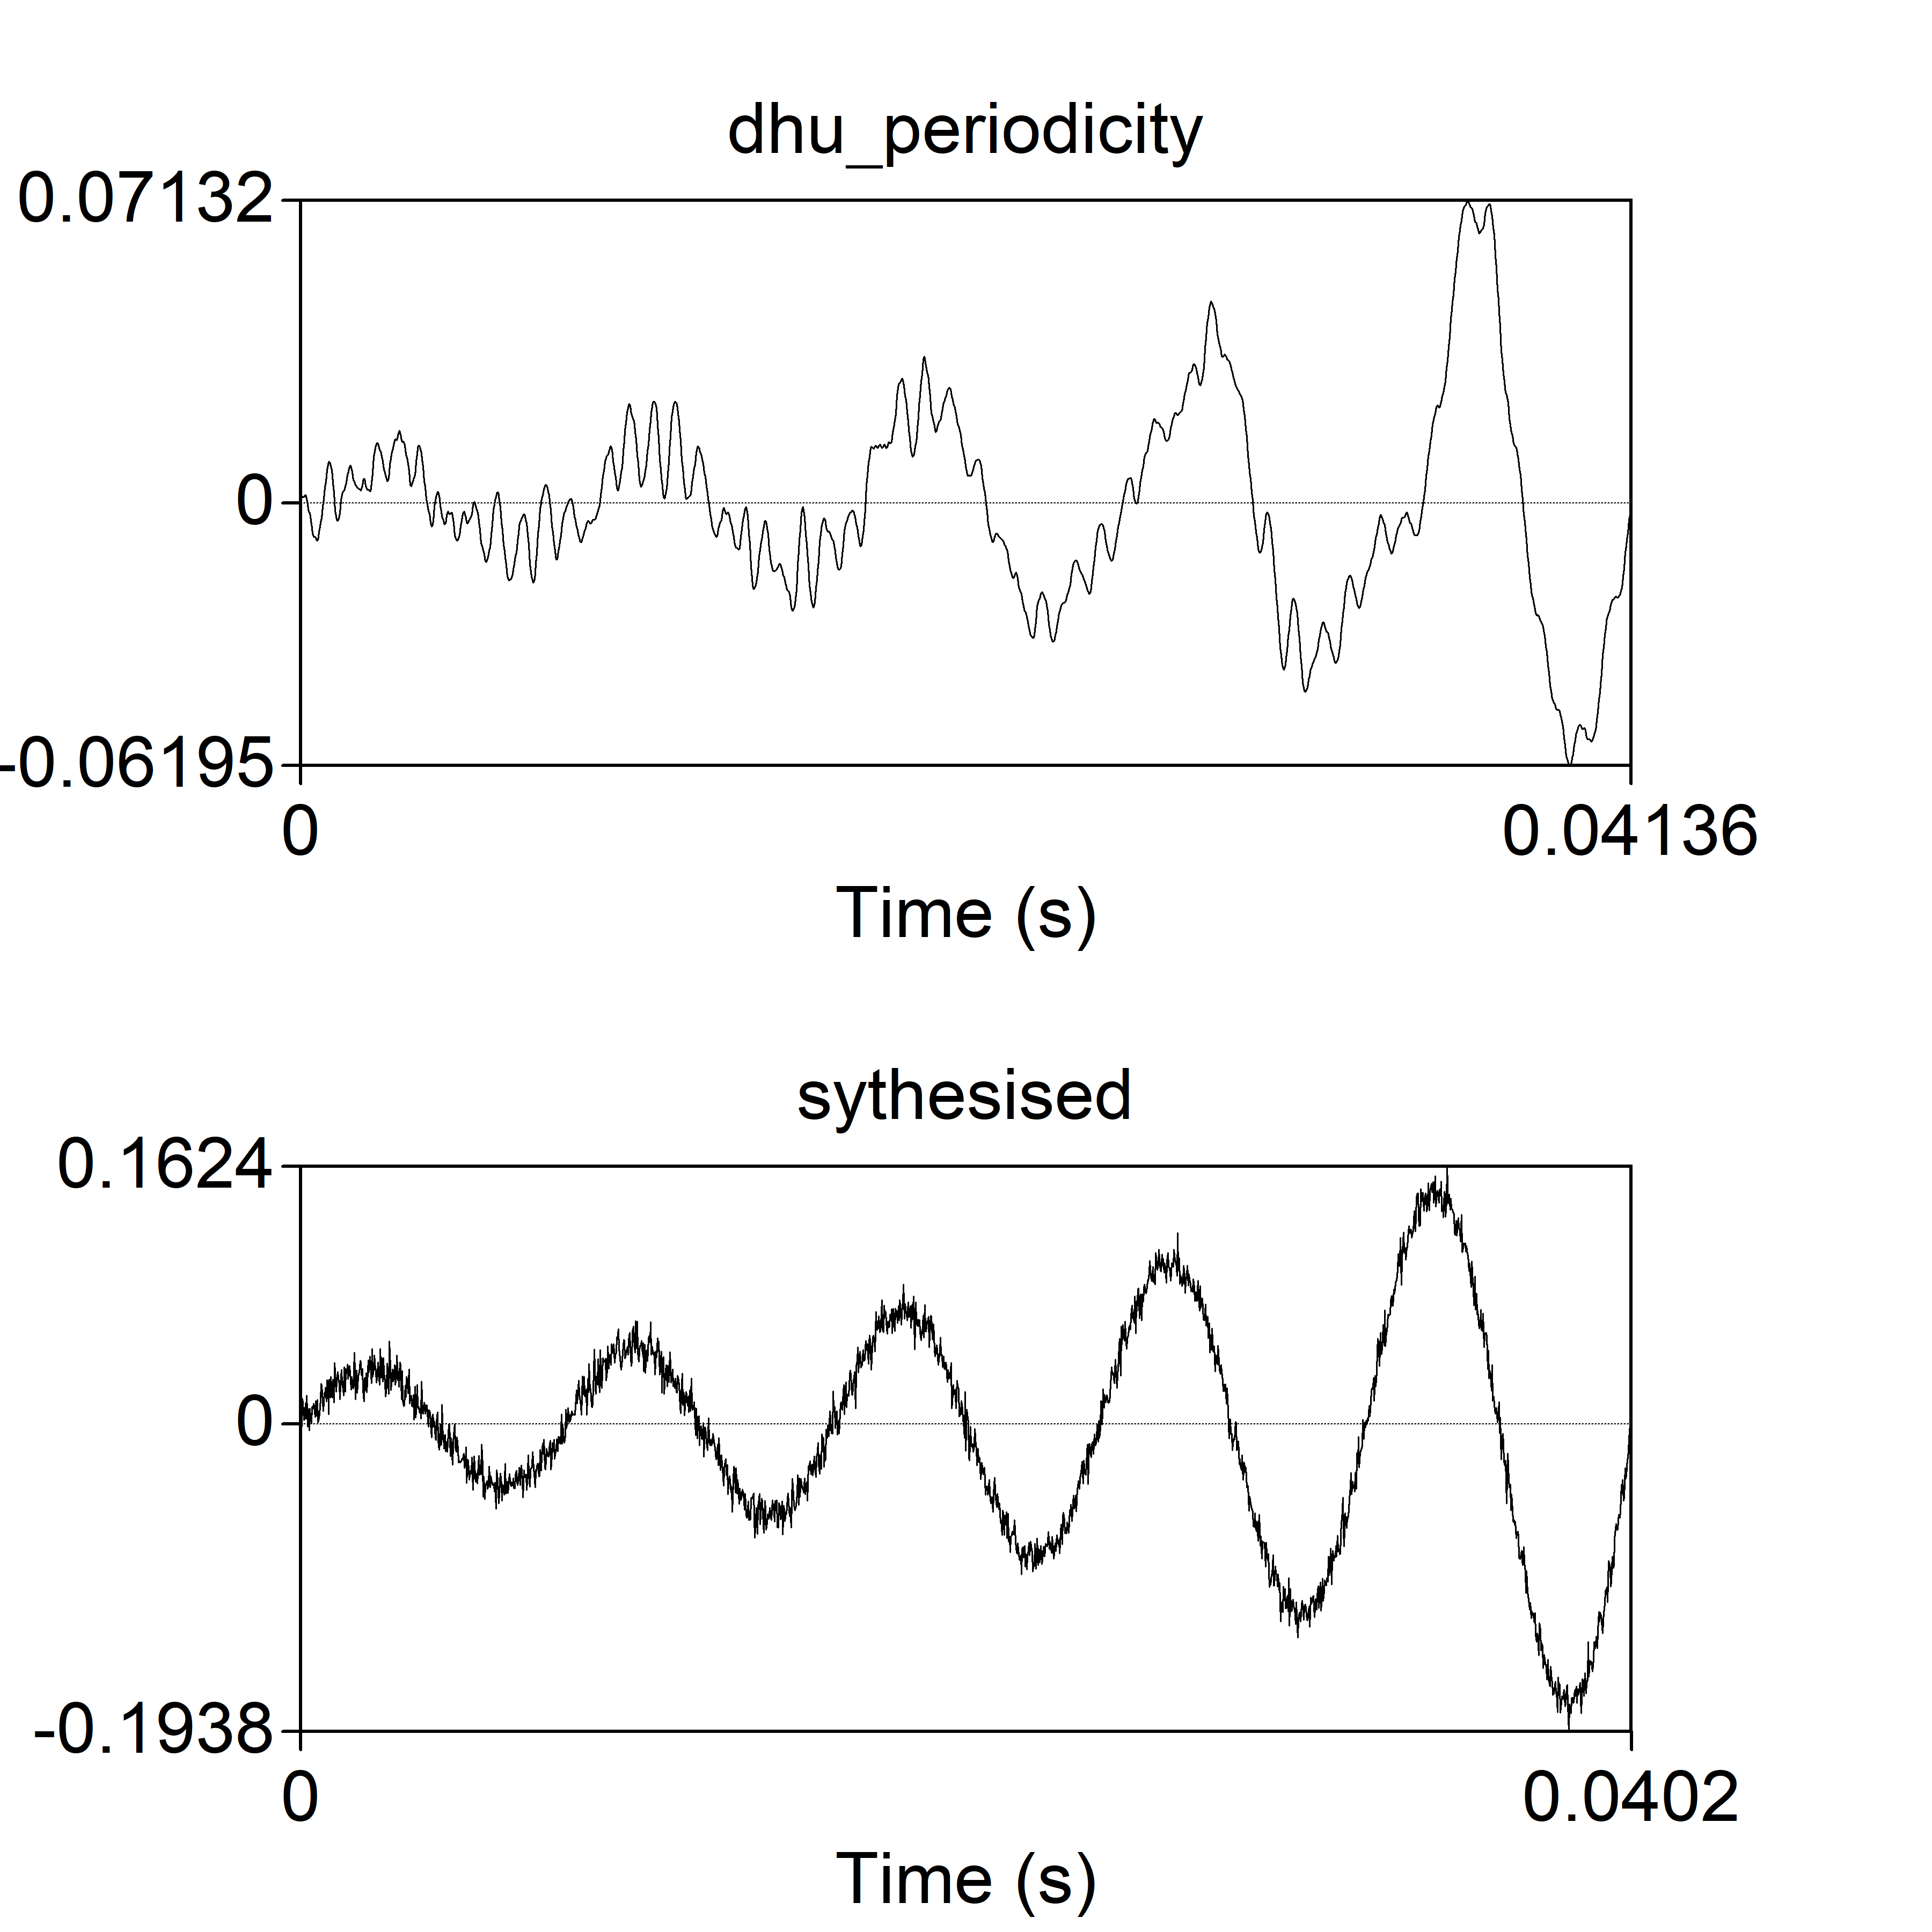
\includegraphics[width=0.5\textwidth]{afterburstpraat.png}
    \caption{Waveforms for periodicity during afterburst to vowel transition in /dh/ (top), synthesised sine wave: attempt to replicate /dh/ afterburst (bottom).}
    \label{fig:afterburst}
\end{figure}

    Intensity was instead manipulated by first cutting the recorded words into three parts: burst, afterburst and rest of the word. The afterbursts of the recorded breathy stop word: \textit{dhuli} (from visible periodicity in afterburst till start of vowel), and recording aspirated stop word: \textit{thukhini} (kept the same duration as the \textit{dhuli} afterburst and with right boundary as start of vowel) were manipulated for intensity. These two were the endpoints for both continua, and intermediate points were manipulated using a multiplying and mixing method. First the endpoint afterbursts were mixed using \textbf{Combine to Stereo} then \textbf{Convert to Mono}, this resulted in an afterburst closer to the breathy afterburst than what was intended (midpoint between aspirated and breathy), this was used as the 6th point for both continua. Reducing the breathy afterburst intensity gave closer results to the aspirated afterburst. The breathy afterburst was multiplied using \textbf{Multiply...} by the factor of 0.3 (30\% of original breathy intensity) to give the 2nd point for both continua, and by the factor of 0.6 (60\% of original breathy intensity) to give the 3rd point for both continua. The same was done for the mixed aspirated-breathy afterburst (6th point) by factors of 0.7 to give the 4th point and 0.75 to give the 5th point. Each manipulated afterburst was put together with the burst and rest of the sound (for both aspirated and breathy) by selecting the three sound objects (it was made sure that object are listed in the order: burst > afterbust > rest, by using \textbf{Copy...}), then \textbf{Concatenate}. \\ \par
    The measurements have been finalised after testing how well a voicing intensity gradient is formed with different multiplying factors, judging this relied on (a)periodicity observation on the afterburst. The increments are not equal like the ones in pitch, and reason for this is that manipulating with equally spaced increments did not result a proper gradient for voicing intensity. However, because the same afterburst points are used for both continua, there is no afterbust voicing intensity differences between the same points across continua. \\ \par
    The manipulation of afterburst voicing intensity does not rely on the manipulation of following vowel pitch and vice-versa, either of the acoustic continua can be created first. The measurements used for each point for both continua are given in Table 1.

\subsection*{Stimuli visualisations} 

\begin{figure}[ht!]

\centering
\subfloat{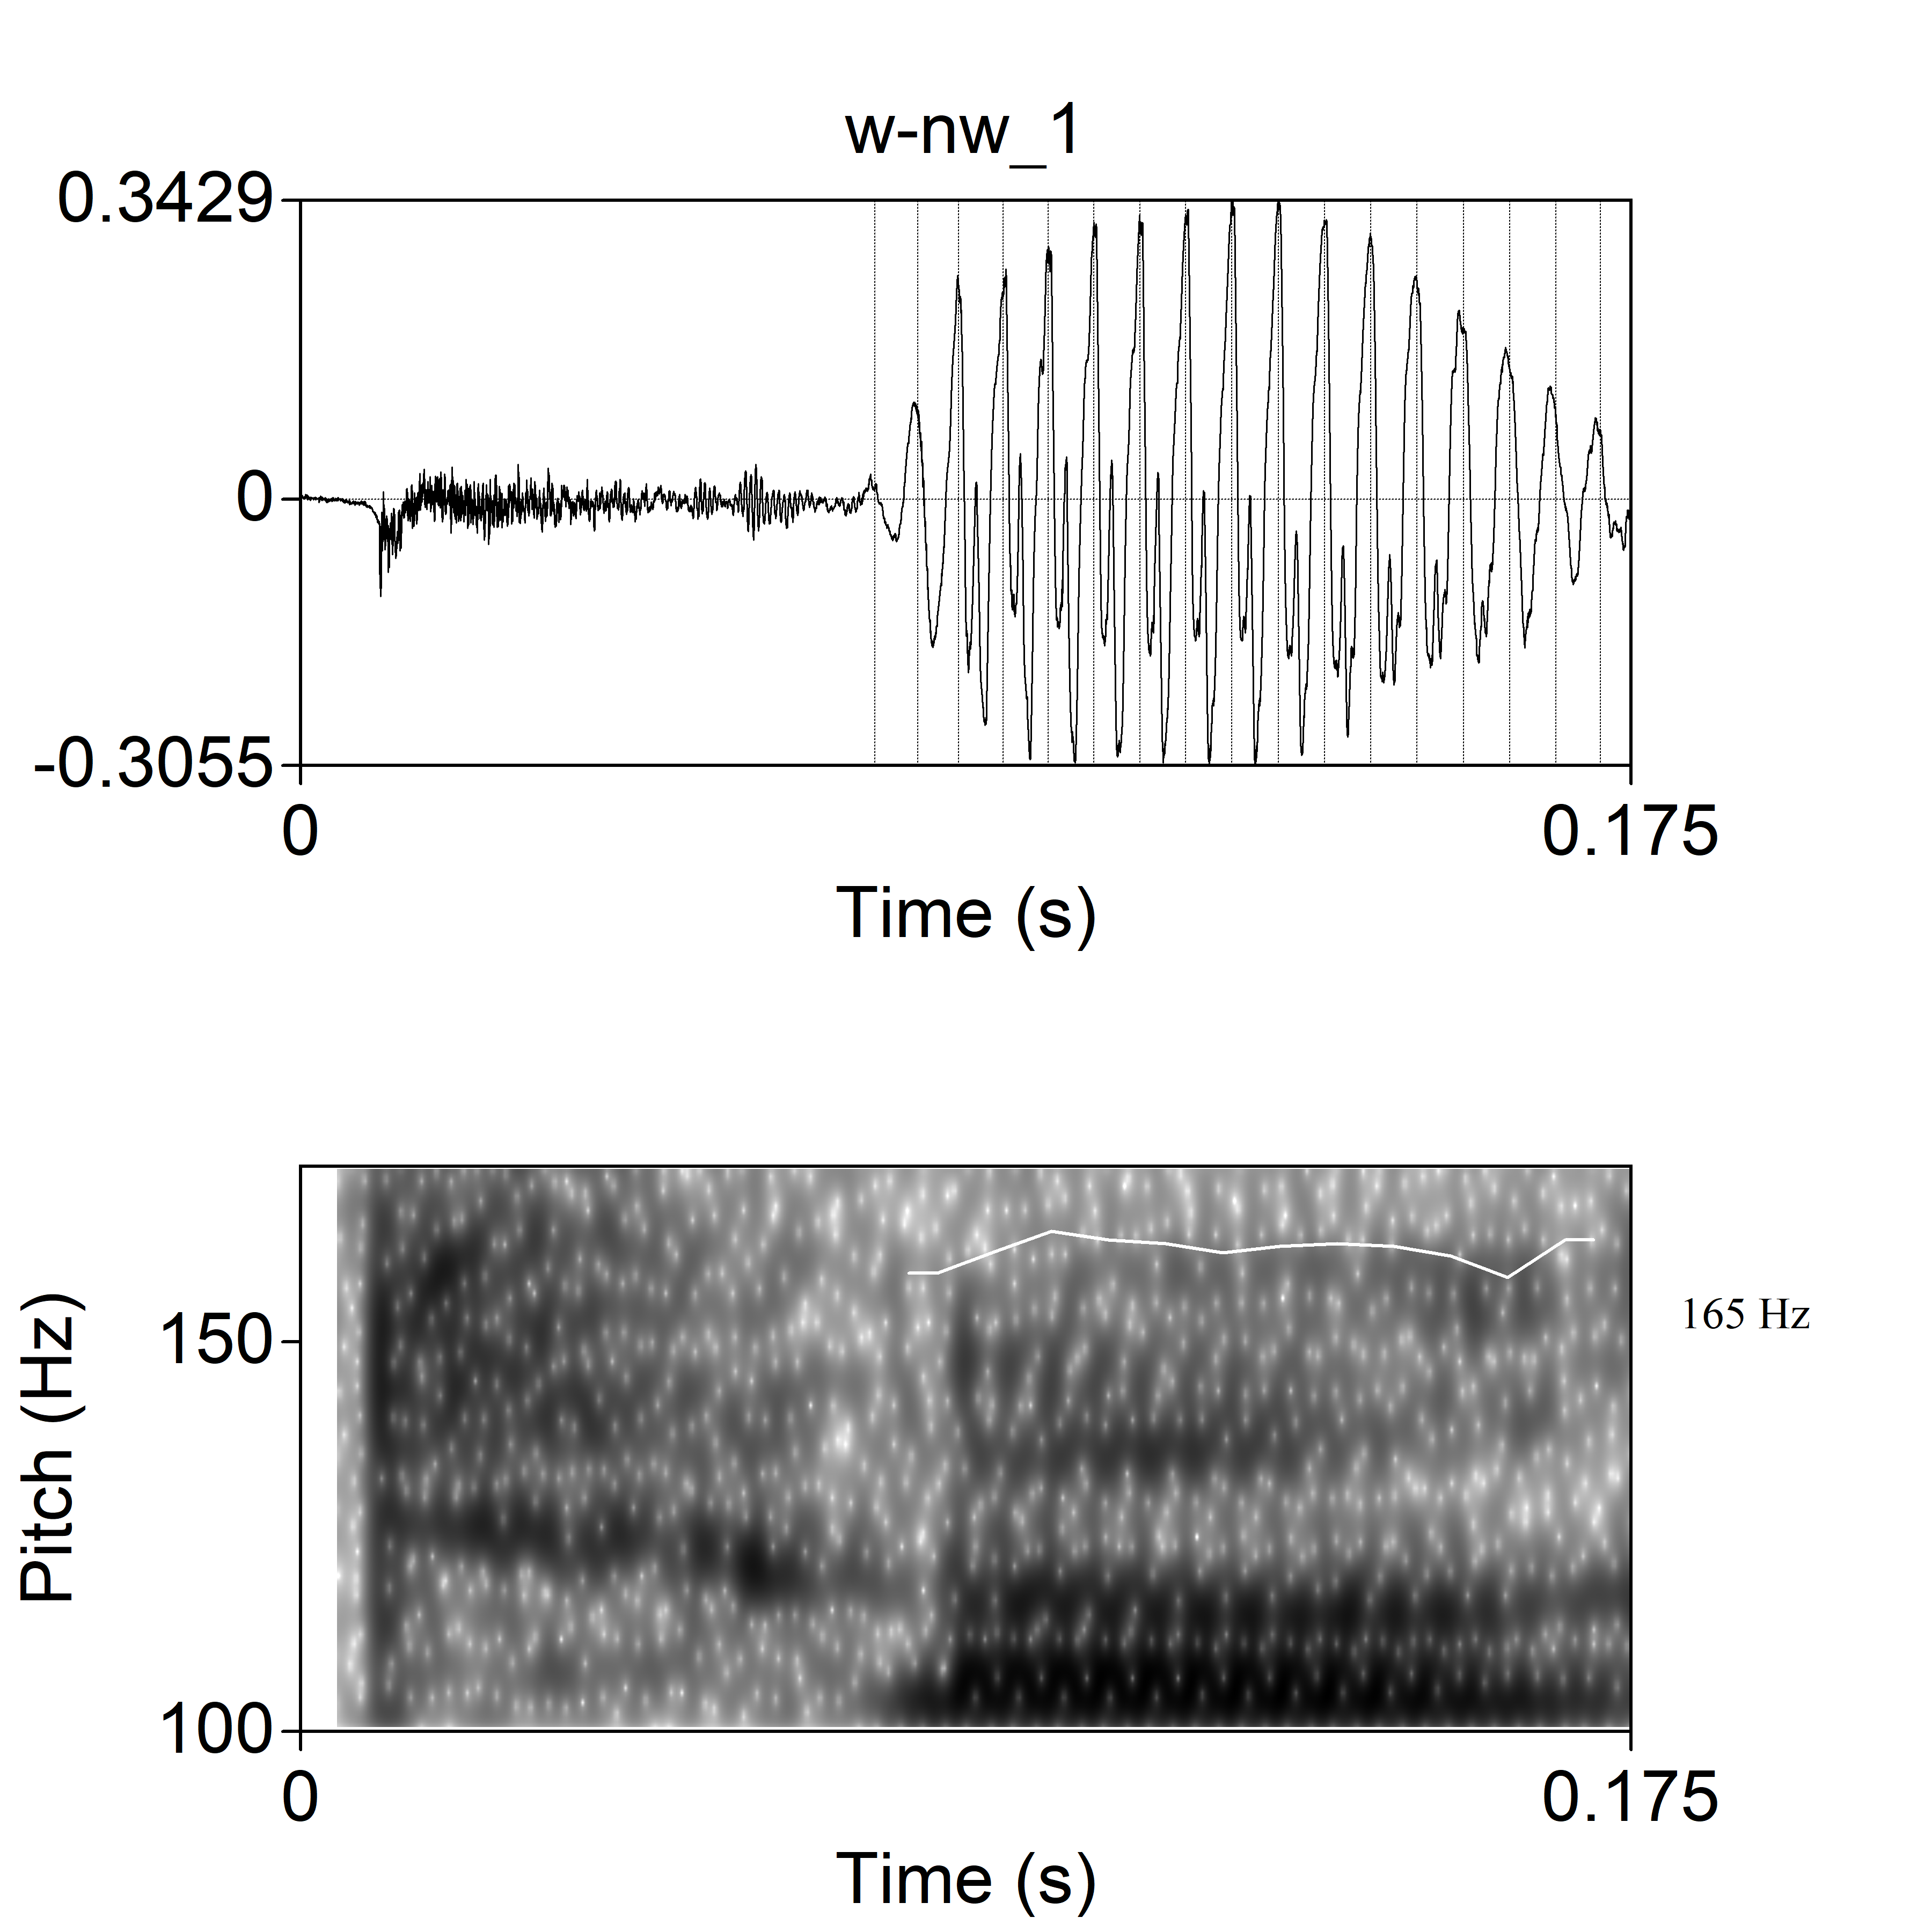
\includegraphics[width=0.5\textwidth]{first.png}\label{fig:viz1}}
\subfloat{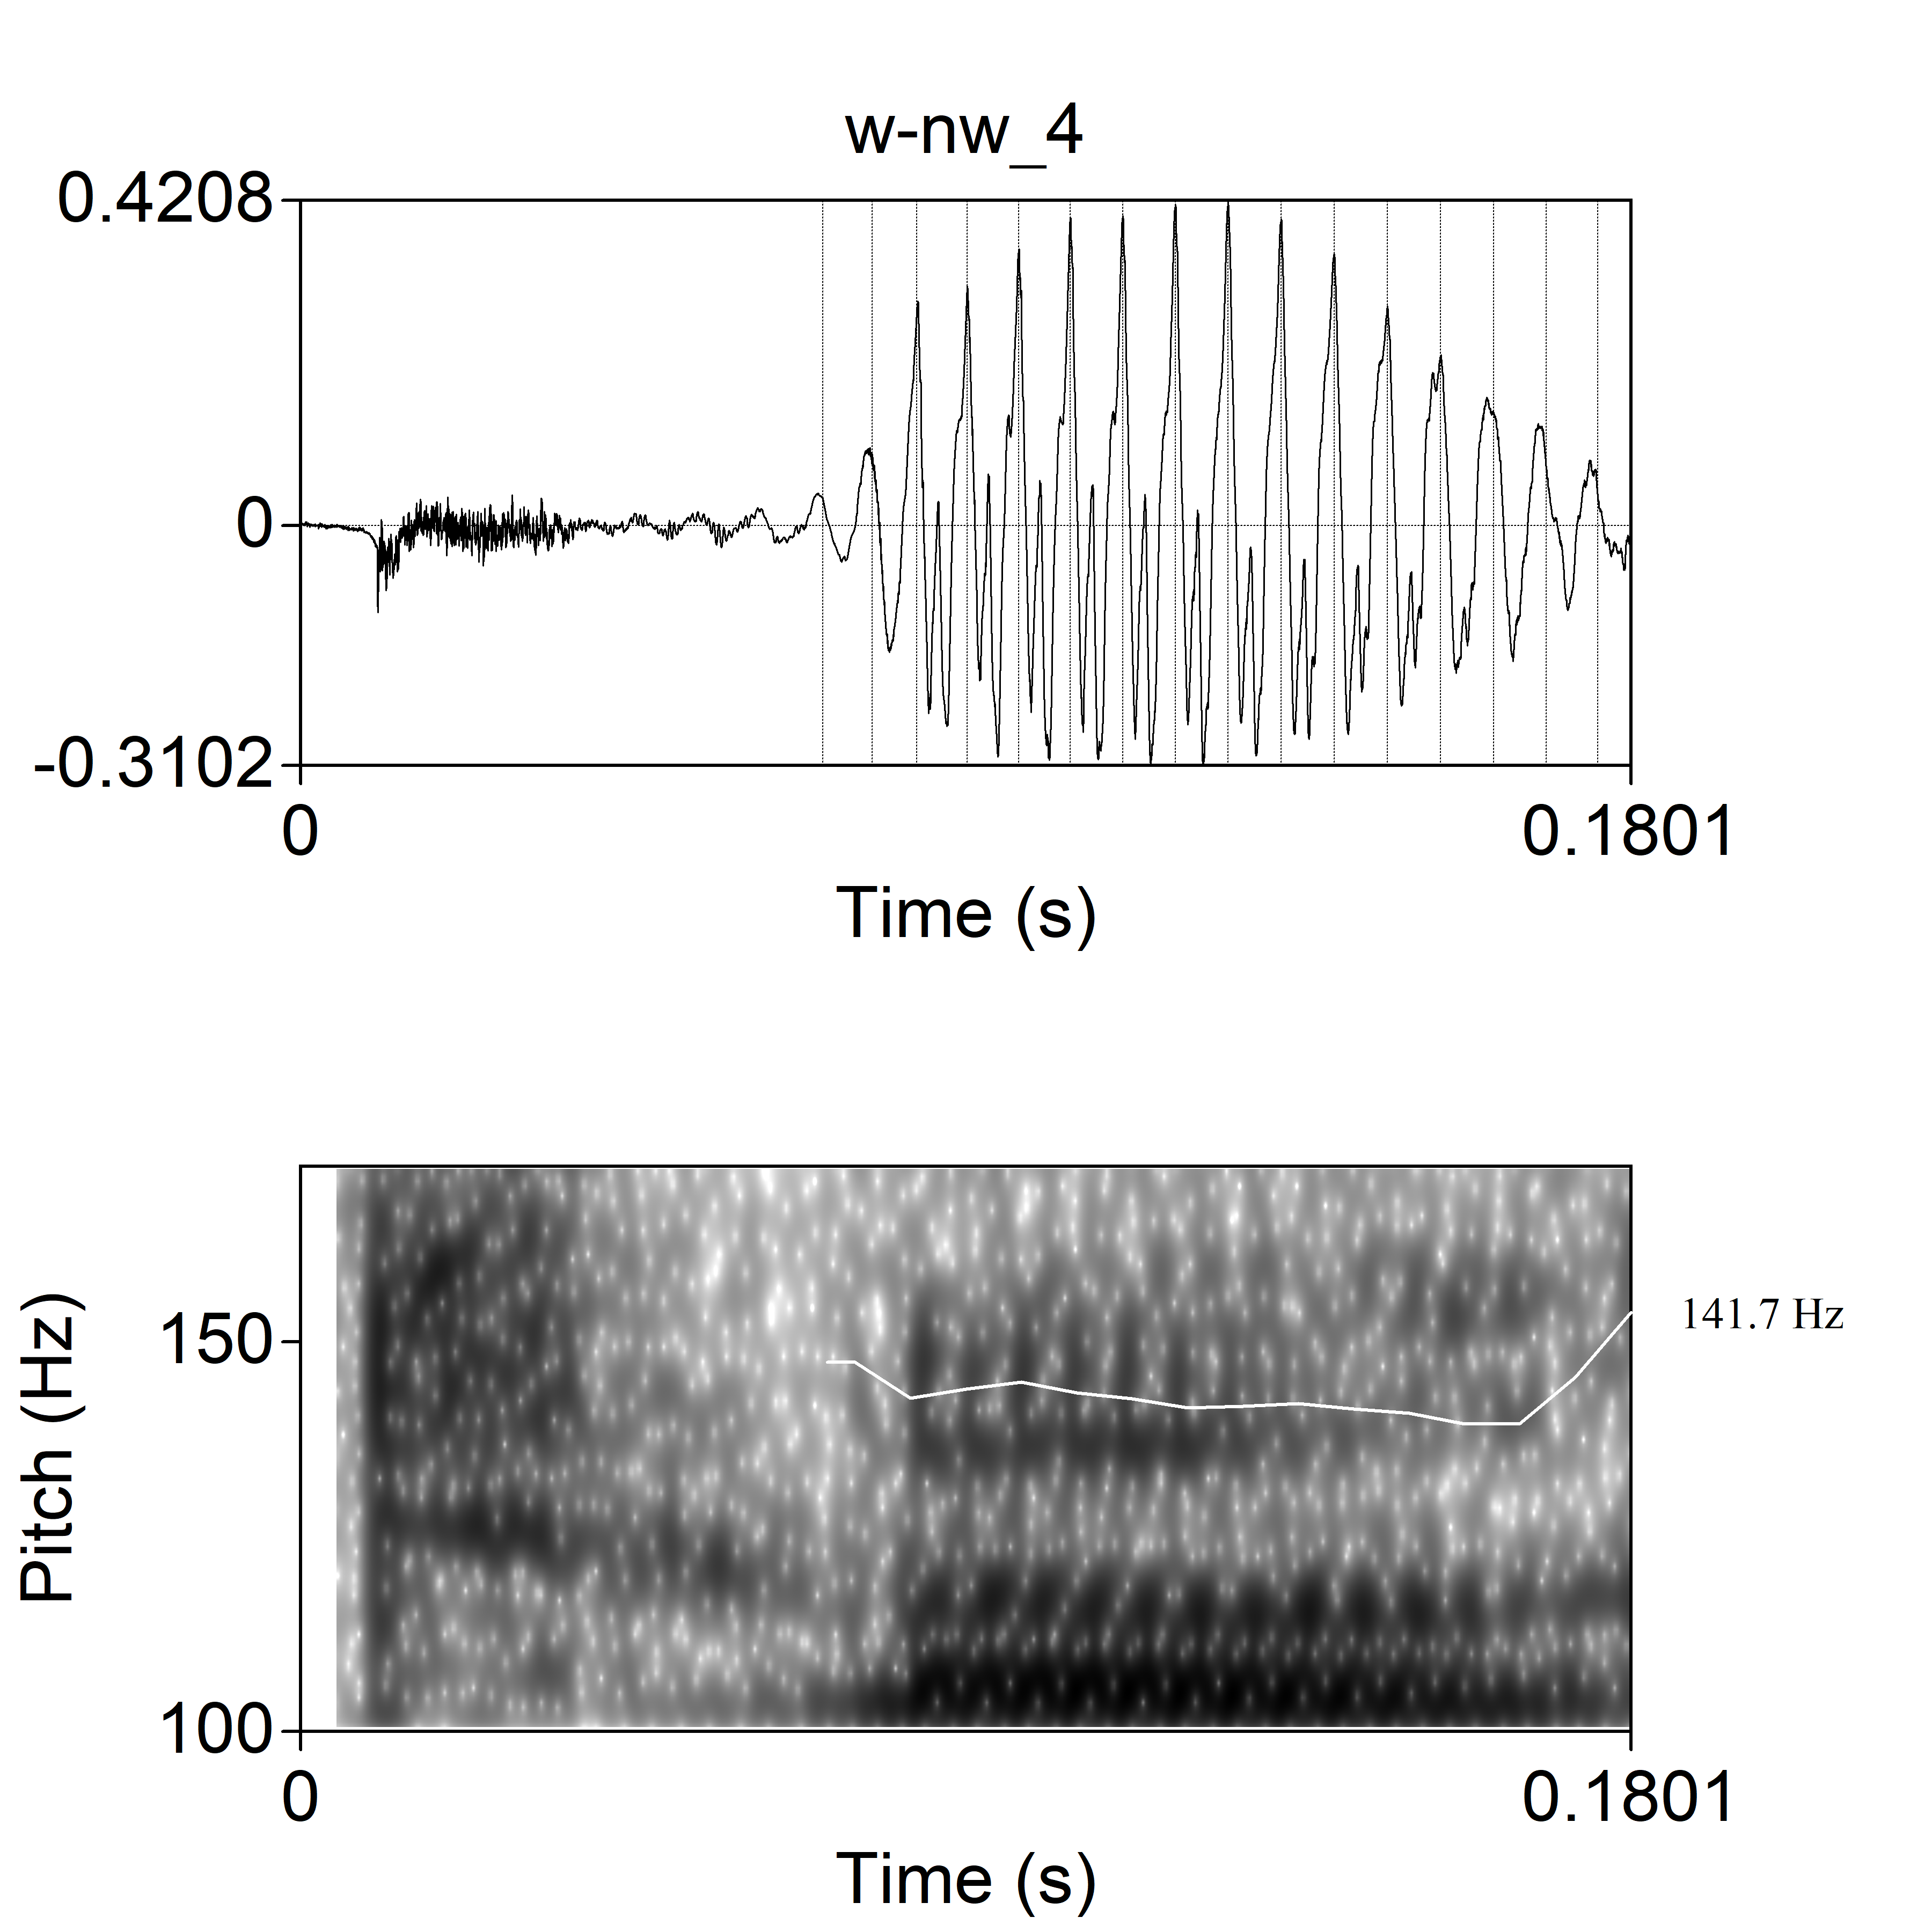
\includegraphics[width=0.5\textwidth]{middle.png}\label{fig:viz2}}\hskip1ex
\subfloat{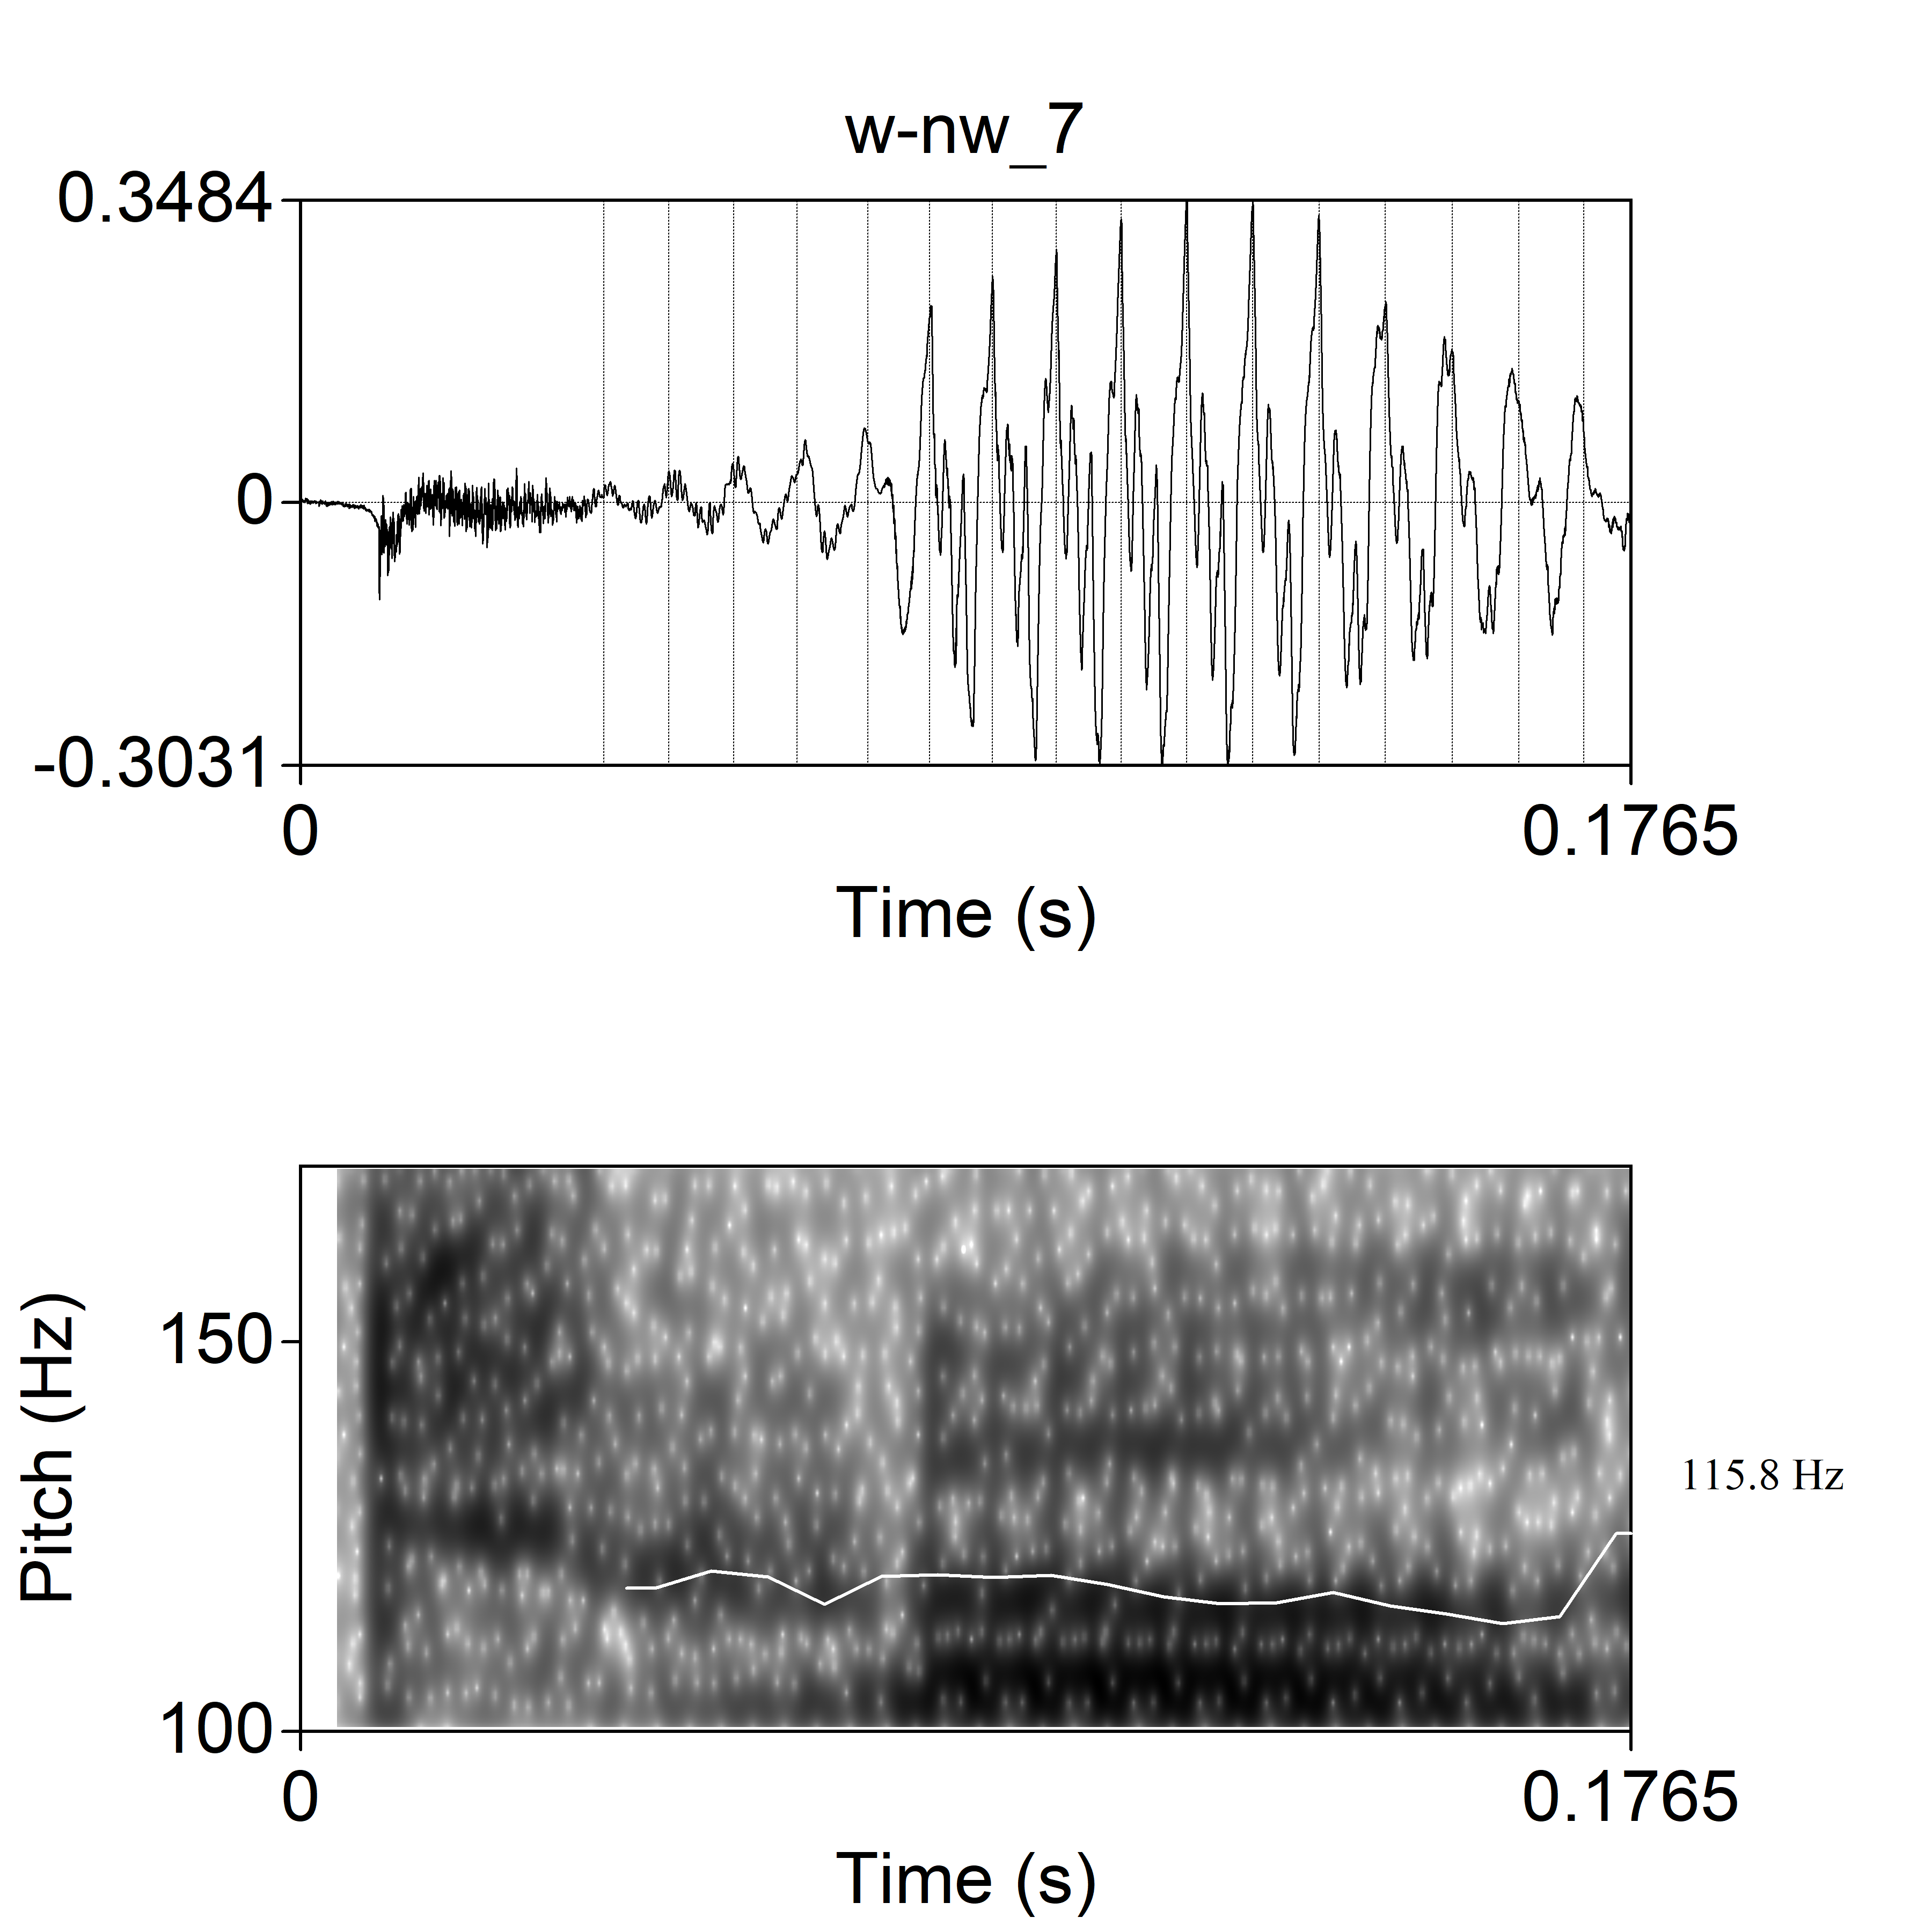
\includegraphics[width=0.5\textwidth]{last.png}\label{fig:viz3}}
\caption{Waveform, pulses, spectrogram, pitch contour and mean pitch for first, fourth, and seventh point in the word-nonword continuum \textit{thukhini-*dhukhini} (only the first syllable is shown)}

\end{figure}

\begin{table}[]

\begin{center}
\begin{tabular}{||m{2cm} m{4cm} m{6cm}||} 
 \hline
 Points (aspirated-breathy) & Indended mean F0 of next vowel (Hz) & Percentage of voicing intencities \\ [0.5ex] 
 \hline\hline
 1 & 165 & 0\% (/th/ afterburst) \\ 
 \hline
 2 & 156.67 & 30\% of /dh/ afterburst \\
 \hline
 3 & 148 & 60\% of /dh/ afterburst \\
 \hline
 4 & 140 & 70\% of mixed afterburst \\
 \hline
 5 & 131.67 & 75\% of mixed afterburst \\
 \hline
 6 & 123.33 & Mixed /dh/ and /th/ afterburst \\
 \hline
 7 & 115 & 100\% (/dh/ afterburst) \\ 
 \hline
\end{tabular}
\end{center}
 \caption{Measurements for pitch and intensity cues for each point in the continua}
\label{tab:measurements}
\end{table}

% ><><><><><><><><><><><><><><><><><><><><><><><><><><><><><

\section*{Results}
\textbf{Analysis Method:} Responses of each participant was stored as Praat ResultsMFC file. These files were selected together to produce a table for all participants. First, this table was extracted as a CSV file, and error responses / double clicks were removed (Appendix 0.4). These were detected as responses with reaction time less than the duration of pre-stimulus sentence, total of four responses were discared. The filtered data was again brought back to Praat and each response was coded for aspirated/breathy with 1 for whichever was selected. The dataset was collapsed to get the sum of aspirated responses for each stimulus. This was again extracted as a CSV, and edited to show percentage of aspirated responses instead (data table in Appendix 0.3), as some stimuli did not have all 120 responses after filtering. Fig. 4 shows the result on graph. \\ \par

\begin{figure}[h!]
    \centering
    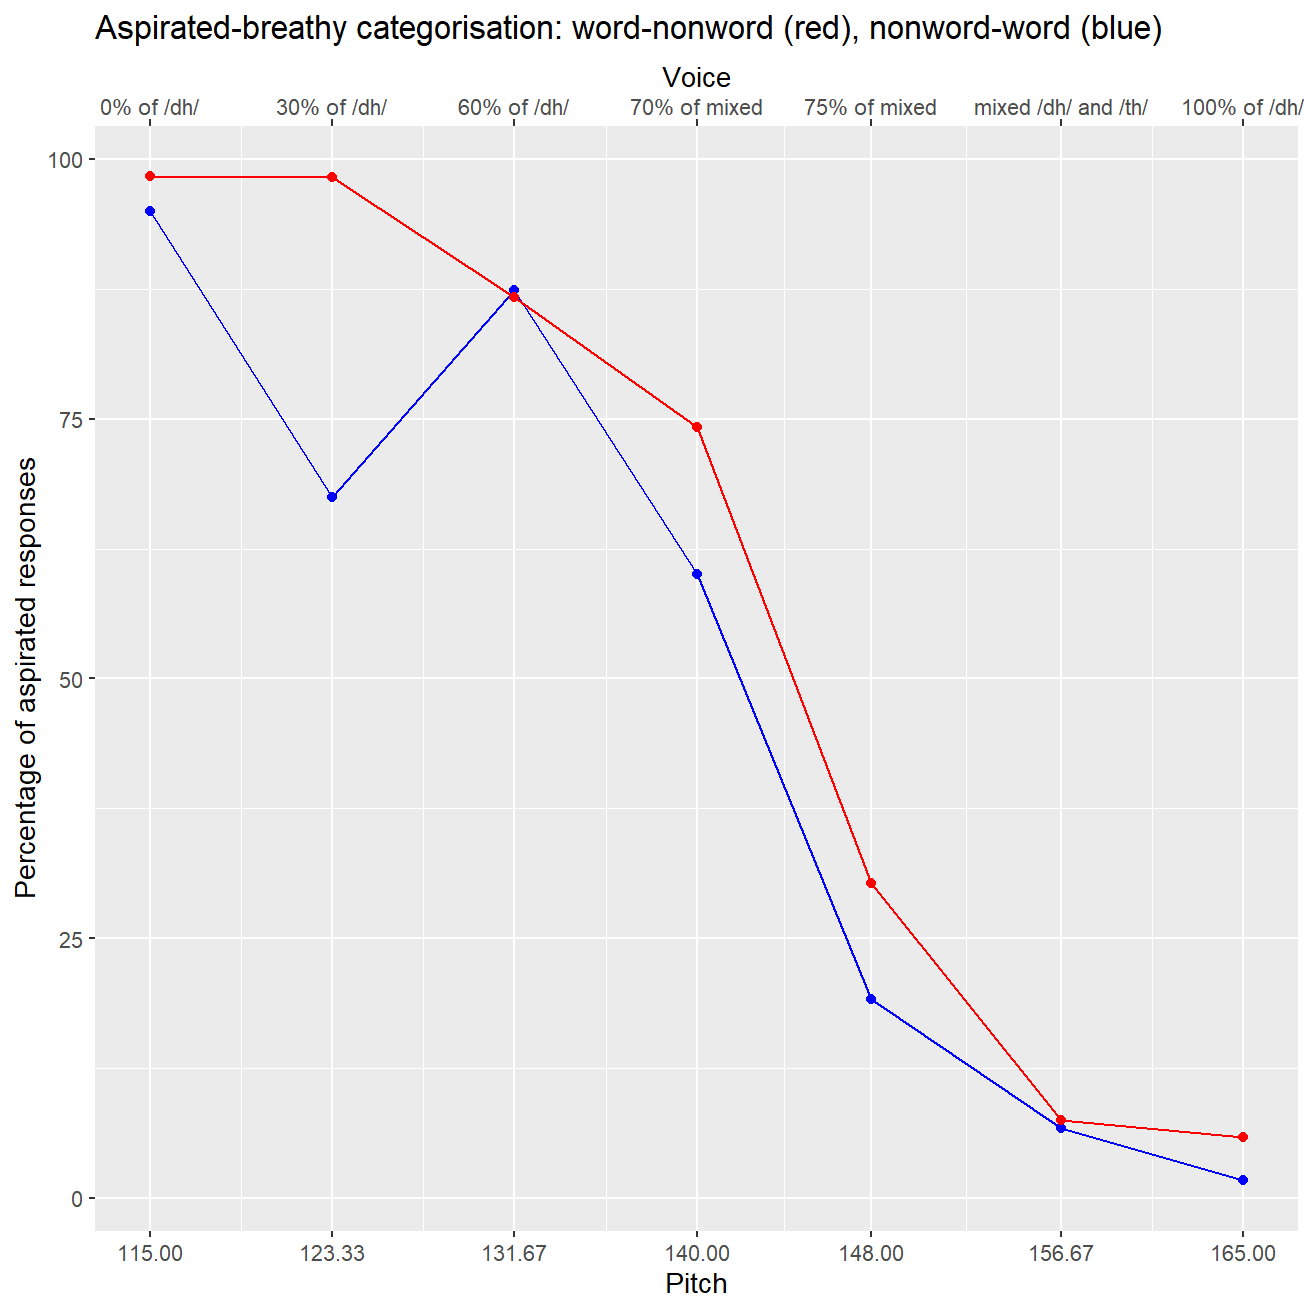
\includegraphics[width=0.6\linewidth]{Rplot02.png}
        \caption{Percentage of aspirated responses over decreasing intended pitch / increasing voicing, for word-nonword (red) and nonword-word (blue) continua. (Note: bottom axis is mistakenly flipped)}
        \label{fig:curves}
\end{figure}

The results show that there was no signficant effect of lexical availability on categorisation of the phonemes on the one-tailed t-test (p = 0.0574, 95\% CI: -4.503m, 34.903, Mean = 15.2, Students' t = 1.745), and also two-tailed t-test (p = 0.1149). Therefore this study cannot conclude existence of lexical effect on phoneme boundary for the tested population. \\ \par

When looking at the graph, there is a clear outlier, nonword-word stimuli 2. But this anomalous point is likely not the source of why results might be insignificant. As the point is rather increasing the difference between the two curves. Elsewhere, the graph seems to be fairly consistent with what is expected from Ganong-effect. The blue line being overall lower than the red line indicates preference for breathy response over aspirated response on the nonword-word continuum, and the opposite preference for the word-nonword continuum. Additionally, increased lexical effect near boundary (points 3 to 6) is noticeable if problematic stimuli is removed along with the previous point (to keep increments consistent). But participants were not tested for just these points, so it should not be considered separately.

% ><><><><><><><><><><><><><><><><><><><><><><><><><><><><><

\section*{Discussion}

The specific research question of this study, if there is lexical effect on phoneme boundary between Assamese breathy and aspirated stops, cannot be confidently answered. As participants did show tendency for lexical effect (especially points 3 to 6), but results are not significant to conclude anything about it. When looking at participants' preference towards one side of the continua, one participant showed complete opposite pattern (favouring /dh/ categorisation for word-nonword, and /th/ categorisation for nonword-word), when excluding results from this participant the results are significant (p < 0.05). However, this significance would most likely arise from the faulty nonword-word stimulus 2 creating a larger gap between the two curves. Moreover, monitoring participants' individual factors like attention span differences is outside the interest of this study, therefore nothing concrete can be said about this participant's responses. \\ \par

There is a possibility that some lexical effect was lost, due to unsureness about non-existence of the nonword stimuli (in literary/formal Asssamese). Some participants expressed that they felt unqualified for the test when asked for participation as their `\textit{likhito} (formal language) is bad' and because the test was on Assamese language they initially formed notions of something like `Assamese language as taught in classroom’ and not the variety they would speak daily. Further, there are factors like the experiment having a test-like setup, where it may be easy to feel like one needs to be correct in some way with their responses. \\ \par


\begin{figure}[t]

\centering
\subfloat{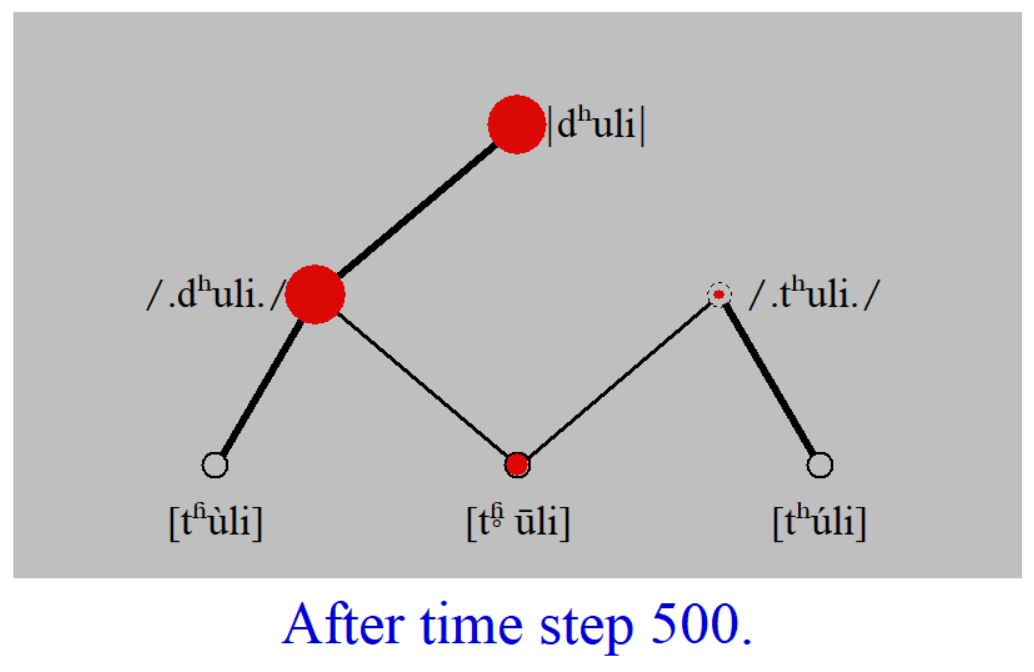
\includegraphics[width=0.3\textwidth]{neural.png}\label{fig:nn}}
\subfloat{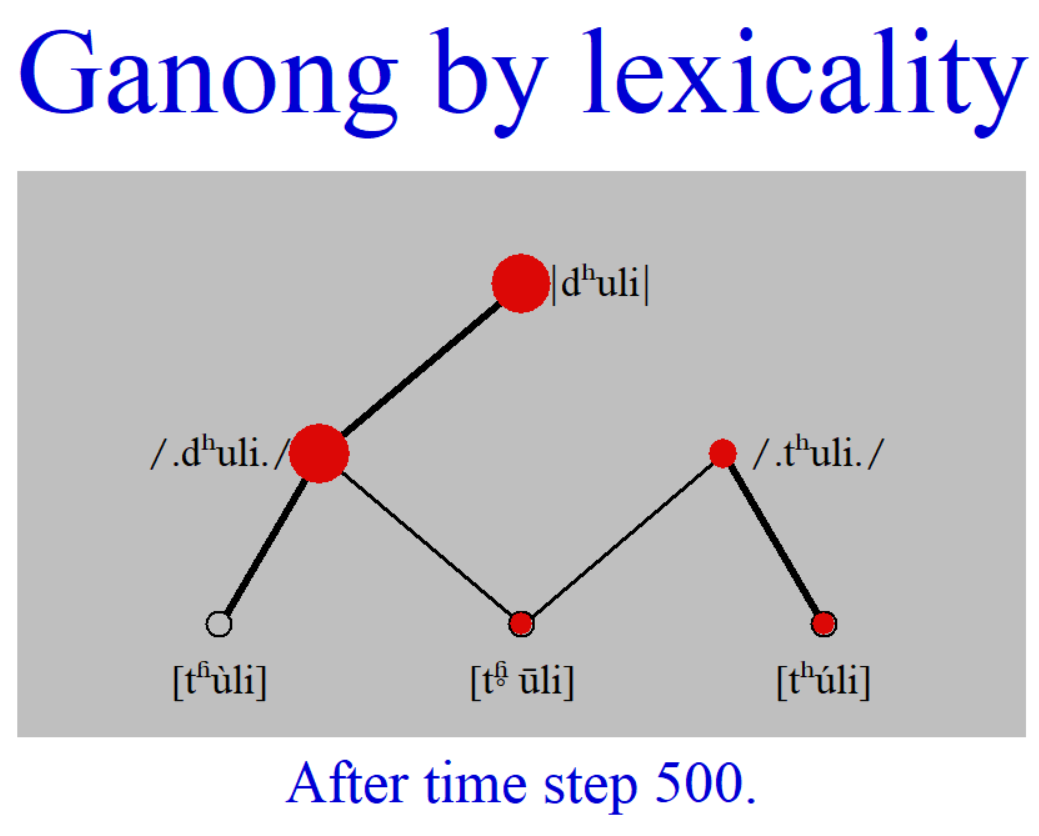
\includegraphics[width=0.3\textwidth]{neural3.png}}\label{fig:nn2}
\subfloat{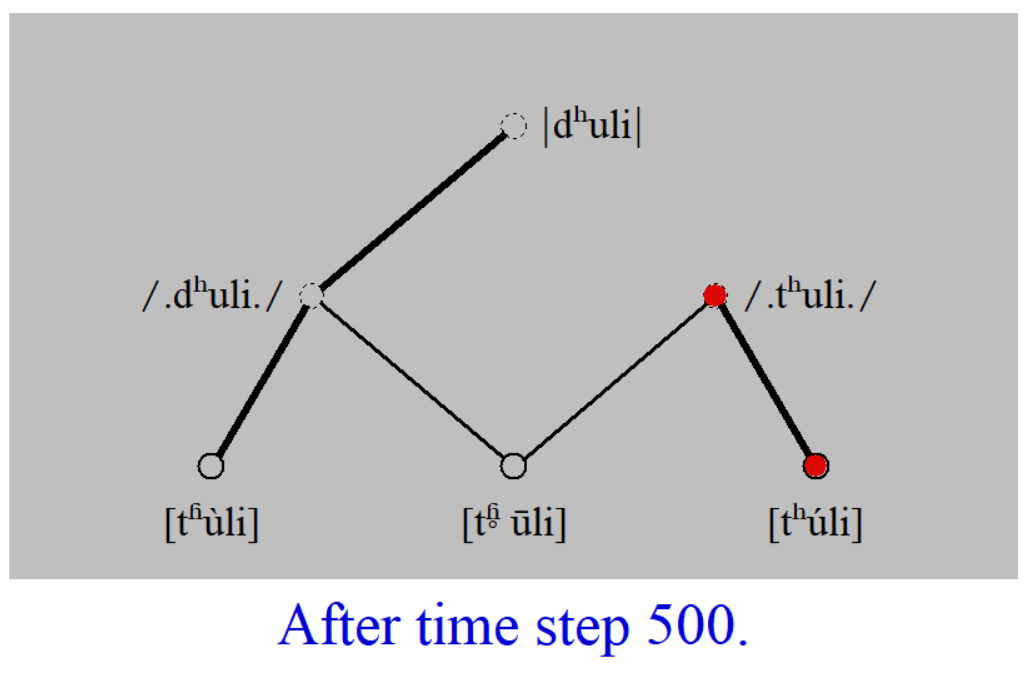
\includegraphics[width=0.3\textwidth]{neural4.png}}\label{fig:nn3}
\caption{Mini neural network displaying how lexical effect can be modelled as realisation close to boundary having better connections to underlying form than a realisation like [thúli].}

\end{figure}

The major problem with this study was not considering influence on percieved pitch from adjescent voiced portions of the sound. Unlike thukhini where /u/ is followed by a voiceless, creating clearer separation for regions where pitch plays a role, the /u/ in dhuli is not. This may indicate something about word level interaction of the pitch cue on aspirated/breathy phonemes. As there is not much (no) work on interaction of following vowel pitch and stops categories with afterburst in Assamese, it was not possible to make judgements for all factors which might be important. \\ \par

Further studies exploring anything related what this study explored, should carry out more investigation on the phonetic nature of categories if not already understood in detail by the literature. For Assamese, more attention to spontaneous and colloquial speech forms is required. There is also a plethora of better experimental design which should be considered: non-remote test, more words on stimuli, filler words during test, better manipulation of the continua, more participants, time, and importantly ensuring participants have no judgement on what or how they must perform in the experiment. What can be done to avoid/study effects from participants' attitudes towards language varieties (like formal Assamese in this case) in their responses, and what other cues are important for stops categories in Assamese (for something like /kh/ and /x/, where the later is often realised as a fricative) are some interesting questions that can be related to this study.


% ><><><><><><><><><><><><><><><><><><><><><><><><><><><><><

\section*{Conclusion}
This study tried to investigate for a phoneme boundary lexical effect between aspirated and breathy phonemes in Assamese using a traditionally undescribed realisation for a breathy stop. Presence for lexical effect cannot be concluded as results are insignificant. There was error in stimuli creation and lack of proper experiment design. Signs of lexical effect are noticeable from the graph otherwise.
% ><><><><><><><><><><><><><><><><><><><><><><><><><><><><><
\bibliographystyle{apalike}
\bibliography{references}
% ><><><><><><><><><><><><><><><><><><><><><><><><><><><><><
\newpage
\section*{Appendices}

\subsection{Praat script}
\begin{itemize}
    \item Finding pitch values of vowel following /dh/ and /th/, and their mean
    \begin{lstlisting}[xleftmargin=0pt]
dhfile$ = "sounds-dh"
thfile$ = "sounds-th"

writeInfoLine: "Average pitch of vowel following dh:"
@pitchAverage: dhfile$
appendInfo: ""
appendInfoLine: "Average pitch of vowel following th:"
@pitchAverage: thfile$

procedure pitchAverage: .file$

	textgridFiles$# = fileNames$# (.file$ +"/*.TextGrid")

	total = 0

	for fileNumber to size (textgridFiles$#)
		textgridFile$ = textgridFiles$# [fileNumber]
		textgrid = Read from file: .file$ +"/" + textgridFile$
		numberOfIntervals = Get number of intervals: 1
		soundFile$ = textgridFile$ - ".TextGrid" + ".wav"
		sound = Read from file: .file$ + "/" + soundFile$
		pitchObject = To Pitch (filtered autocorrelation): 0, 50, 800, 15, "yes", 0.03, 0.09, 0.5, 0.055, 0.35, 0.14
	
		for interval to numberOfIntervals
			selectObject: textgrid
			text$ = Get label of interval: 1, interval
			if text$ = "v"
				start = Get start time of interval: 1, interval
				end = Get end time of interval: 1, interval
				selectObject: pitchObject
				pitch = Get mean: start, end, "Hertz"
			endif
		endfor
		appendInfoLine: pitch
		total = total+pitch
		removeObject: textgrid, sound, pitchObject
	endfor
	average = total / size(textgridFiles$#)
	appendInfoLine: ""
	appendInfoLine: fixed$ (average, 1), newline$
endproc
    \end{lstlisting}
\end{itemize}

\subsection{Experiment file}
\begin{itemize}
    \item 
    \begin{lstlisting}[xleftmargin=0pt]
"ooTextFile"
"ExperimentMFC 7"

blankWhilePlaying? <no>
stimuliAreSounds? <yes>
stimulusFileNameHead = "working/"
stimulusFileNameTail = ".wav"
stimulusCarrierBefore = "before" ; file name of the recording before the file: manu tue koise
stimulusCarrierAfter = "" ; file name of the recording after
stimulusInitialSilenceDuration = 0.5 seconds
stimulusMedialSilenceDuration = 0
stimulusFinalSilenceDuration = 0.5 seconds
numberOfDifferentStimuli = 14 ; number of total stimuli then after this line there are file names (eg here is of length)
    "w-nw_1"  ""
    "w-nw_2"  ""
    "w-nw_3"  ""
    "w-nw_4"  ""
    "w-nw_5"  ""
    "w-nw_6"  ""
    "w-nw_7"  ""
    "nw-w_1"  ""
    "nw-w_2"   ""
    "nw-w_3"   ""
    "nw-w_4"   ""
    "nw-w_5"   ""
    "nw-w_6"   ""
    "nw-w_7"   ""

numberOfReplicationsPerStimulus = 12
breakAfterEvery = 40
randomize = <PermuteBalancedNoDoublets>
startText = "This is a listening experiment.
After hearing, you choose the sound that is most similar.

Click to start."
runText = "Choose the sound that you heard."
pauseText = "You can have a short break if you like.

Click to proceed."
endText = "The experiment
has finished."
maximumNumberOfReplays = 0
replayButton = 0 0 0 0 "" ""
okButton = 0 0 0 0 "" ""
oopsButton = 0 0 0 0 "" ""

responsesAreSounds? <no> "" "" "" "" 0 0 0
numberOfDifferentResponses = 2
    0.25 0.45 0.4 0.6 "ধ্ / dh" 40 "" "dh"
    0.55 0.75 0.4 0.6 "থ্ / th" 40 "" "th"

numberOfGoodnessCategories = 0
    \end{lstlisting}
\end{itemize} \newpage

\subsection{Resulting data file}

% Please add the following required packages to your document preamble:
% \usepackage{graphicx}
\begin{table}[h]
\resizebox{\textwidth}{!}{%
\begin{tabular}{llllllll}
stimulus & nw-w\_num & w-nw\_num & nw-w\_perc & w-nw\_erc & points & pitch & voice \\
nw-w\_1 & 114 & 118 & 95 & 98.3333 & 1 & 115 & 0\% of /dh/ \\
nw-w\_2 & 81 & 116 & 67.5 & 98.3051 & 2 & 123.33 & 30\% of /dh/ \\
nw-w\_3 & 104 & 104 & 87.395 & 86.6667 & 3 & 131.67 & 60\% of /dh/ \\
nw-w\_4 & 72 & 89 & 60 & 74.1667 & 4 & 140 & 70\% of mixed \\
nw-w\_5 & 23 & 36 & 19.1667 & 30.2521 & 5 & 148 & 75\% of mixed \\
nw-w\_6 & 8 & 9 & 6.6667 & 7.5 & 6 & 156.67 & mixed /dh/ and /th/ \\
nw-w\_7 & 2 & 7 & 1.6667 & 5.8333 & 7 & 165 & 100\% of /dh/
\end{tabular}%
}
\caption{}
\label{tab:my-table}
\end{table}

\subsection{R commands used to analyse results}
\begin{itemize}
    \item Removing error responses
    \begin{lstlisting}[xleftmargin=0pt]
library(tidyverse)
allResults_filtered <- filter(allResults, reactionTime >= 1.3)
    \end{lstlisting} \vspace{10pt}
    \item Graph plot
    \begin{lstlisting}[xleftmargin=0pt]
library(tidyverse)
ggplot() + 
  geom_line(data = byStimulus_final, mapping = aes(x=pitch, y=right1), color="blue")+
  geom_point(data = byStimulus_final, mapping = aes(x=pitch, y=right1), color="blue")+
  geom_line(data = byStimulus_final, mapping = aes(x=pitch, y=right2), color="red")+
  geom_point(data = byStimulus_final, mapping = aes(x=pitch, y=right2), color="red")+
  scale_x_continuous(
    breaks = byStimulus_final$pitch,
    name = "Pitch",
    sec.axis = dup_axis(name = "Voice",
                        labels = byStimulus_final$voice))+
  labs(x = "Pitch", 
       y = "Percentage of aspirated responses", 
       title = "Aspirated-breathy categorisation: word-nonword (red), nonword-word (blue)")
    \end{lstlisting}
\end{itemize}

\subsection{Ethics material}
Ethics materials are attached with this file.

%wwwwwwwwwwwwwwwwwwwwwwwwwwwwwwwwwwwwwwwwwwwwwwwwwwwwwwwww
\end{document}